\label{sec:4.1}

%%%%%%%%%%%%%%%%%%%%%%%%%%%%%%%%%%%%%%%%%%%%%%%%%%%%%%%
%(GAO) Discuss noise performance
%%%%%%%%%%%%%%%%%%%%%%%%%%%%%%%%%%%%%%%%%%%%%%%%%%%%%%%
The key performance metric for the ColdADC is its noise performance, as it directly impacts the 
sensitivity of the experiment. The design goal for the ColdADC was for its internal noise to be well 
below the noise of the LArASIC, so the LArASIC would dominate the overall noise of the system. 
This has been achieved as the ADC met its goal of 200 $\mu$V-rms noise at LN$_2$ temperature. 
Detailed measurements of the ASIC and system noise in different conditions follow.

\subsubsection{ColdADC Only}
The noise distribution for 16-channels from one ColdADC chip with the input floating are shown in Figure~\ref{fig:qc_noisewarm} (RT) and Figure~\ref{fig:qc_noisecold} (LN$_2$). The results are given in full 16-bit ADC output. The average noise is 6.7 LSB (302 $\mu$V-rms) at warm and 4.2 LSB (189 $\mu$V-rms) in LN$_2$, in 16-bit. The measurement is done with ColdADC configured after calibration, VDDA2P5/VDDD2P5=2.5 V, VDDD1P2=2.0 V, VDDIO=2.25 V, SDC bypassed. Separate study has shown that SDC noise is negligible. 
\begin{figure}[h!]
\centering
  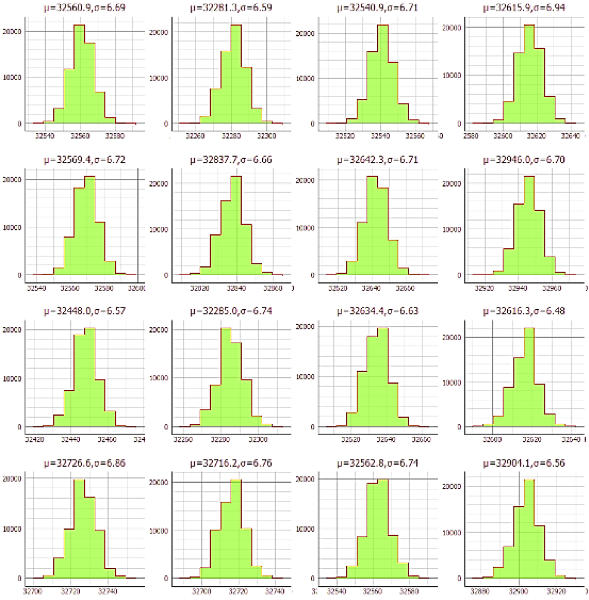
\includegraphics[width=0.8\linewidth]{figures/qc_noisewarm.png}
  \caption{Noise distribution (16-bit) of 16 input channels at room temperature.}
  \label{fig:qc_noisewarm}
\end{figure}
\begin{figure}[h!]
\centering
  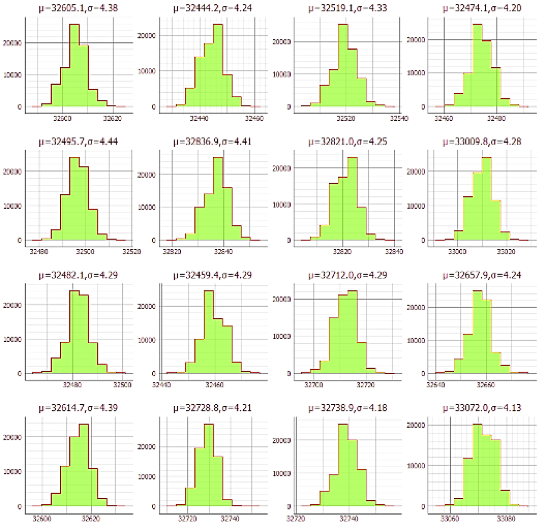
\includegraphics[width=0.8\linewidth]{figures/qc_noisecold.png}
  \caption{Noise distribution (16-bit) of 16 input channels at LN$_2$ temperature.}
  \label{fig:qc_noisecold}
\end{figure}

\subsubsection{LArASIC + ColdADC}
To evaluate the combined noise of LArASIC and ColdADC, 150pF mica capacitor is added to the LArASIC input 
to simulate the capacitance of the detector sense wire. 
Noise characterization is made at both room and LN2 temperatures, as shown in Figure~\ref{fig:noise_fullchain}.  
The quantization noise of 12-bit ADC is negligible when LArASIC gain is set to 7.8 mV/fC or higher.
With a shaping time $>$ 2 $\mu$s, the ENC noise is below 630 e$^-$ at RT and $<$ 500 e$^-$ at LN$_2$ temperature.
\begin{figure}[h!]
\centering
  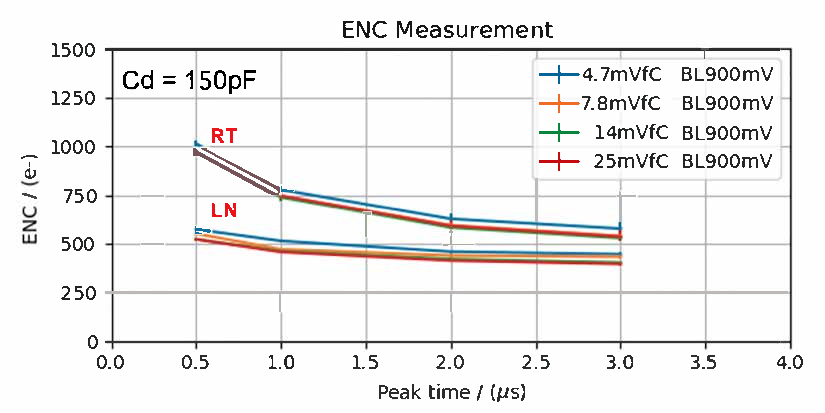
\includegraphics[width=0.8\linewidth]{figures/noise_fullchain.pdf}
  \caption{LArASIC + ColdADC (12-bit mode) noise as a function of shaping time at RT and LN$_2$ temperatures.}
  \label{fig:noise_fullchain}
\end{figure}

The noise dependence on the input capacitance is also studied. In this setup, each input LArASIC channel has
a different capacitor with value that ranges from 22 pF to 150 pF. The input capacitance dependence result in 
LN$_2$ is shown in Figure~\ref{fig:noise_capacitance} . The four different curves correspond 
to different values of LArASIC shaping time. 
The noise performance comparison between ColdADC BGR and CMOS reference, and comparison between 
SDC and bypassing SDC show no significant difference.
The ENC noise performance for the LArASIC + ColdADC setup has better noise performace compared to 
MicroBooNE, ProtoDUNE, and SBND cold electronics (see results in the Appendix).
\begin{figure}[h!]
\centering
  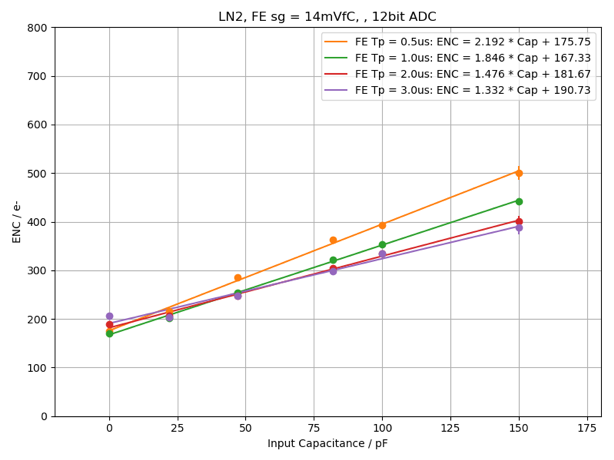
\includegraphics[width=0.8\linewidth]{figures/noise_capacitance.png}
  \caption{ENC vs. input capacitance at LN$_2$ temperature. LArASIC is configured with a gain setting of
14 mV/fC, ColdADC output is trucated to 12-bit. The four curves corresponds to (from to to bottom) 0.5, 
1.0, 2.0, and 3.0 $\mu$s shaping time.} 
  \label{fig:noise_capacitance}
\end{figure}

The DUNE requirement calls for a 12-bit ADC. The nominal plan is to trucate 16-bit ColdADC output down to 
12-bit. Given the low noise of the ColdADC, we explore the feasibility of outputing more than 12-bit.
Earlier Figure~\ref{fig:noise_fullchain} demonstrates that when LArASIC gain is set to 7.8 mV/fC or higher, 
the quantitization noise of 12-bit ADC is negligible. Figure~\ref{fig:noise_quant150pf} 
shows the ENC as a function of shaping time for 16, 14, and 12 bit ADC output with input LArASIC capacitance
of 150 pF. Figure~\ref{fig:noise_quantfloat} shows the ENC with LArASIC input floating. With the 
current noise performance, the quantization noise is negligible at 14-bit output even with the lowest LArASIC gain setting of 4.7 mV/fC.
\begin{figure}[h!]
\centering
  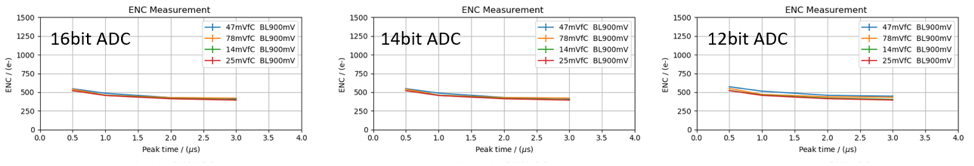
\includegraphics[width=1.0\linewidth]{figures/noise_quant150pf.png}
  \caption{ENC vs. Shaping Time at LN$_2$ temperature. Input capacitance is 150 pF. Different curves 
correspond to gain setting of (top to bottom) 4.7, 7.8, 14, 25 mV/fC.}
  \label{fig:noise_quant150pf}
\end{figure}
\begin{figure}[h!]
\centering
  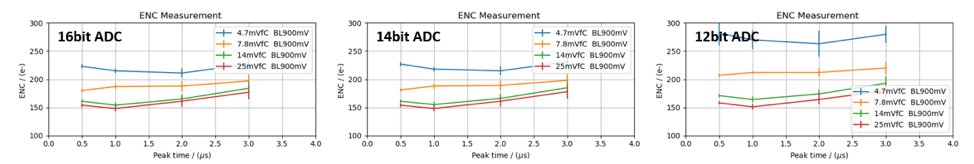
\includegraphics[width=1.0\linewidth]{figures/noise_quantfloat.png}
  \caption{ENC vs. Shaping Time at LN$_2$ temperature. Input floating. Different curves correspond to 
gain settings of (top to bottom) 4.7, 7.8, 14, 25 mV/fC.}
  \label{fig:noise_quantfloat}
\end{figure}



